{\textbf{可能疑问点:我是零基础的跨专业考生,要不要先看数字电路等基础知识?直接看计算机组成原理教材可以理解吗?}}

解答:想必以上问题是95\%跨专业考生必问的。当然,两年前编者作为零基础的跨专业考生,也问过类似的问题。现在编者以一个过来者的身份很肯定地回答你:只需学习一些基础的辅助知识(考研的范围要求)。

\textbf{在讲解考研知识点之前,}此书先给读者介绍一些计算机组成原理的辅助知识,在以后的讲解中就不再重复了。

\subsection{\texorpdfstring{{入门知识}{1}{:了解门电路}}{入门知识1:了解门电路}}\label{ux5165ux95e8ux77e5ux8bc61ux4e86ux89e3ux95e8ux7535ux8def}

在考研知识范围内,门电路不会考查得很复杂,考生只需了解几个基本的门电路即可。

顾名思义,``门''起到开关的作用,如某公司要招聘员工,公司对待招聘员工的要求是既要有技术,又要沟通能力好,因此只要应聘的人同时满足这两个要求就有可能被公司录用。然而,不同的公司对员工有不同的要求,如另外一家公司可能只要技术和沟通能力满足其一即可,那么又可以形成新的``门''。同理,在计算机中,如果有多个输入端,此``门''就可以对这些输入端``提出''要求,如每个输入端都是高电平,``门''才打开;或者多个输入端只要有一个是高电平,``门''就打开。以上就是门电路的基本涵义。

\textbf{下面介绍常用的6种门电路,}以下假设都只有两个输入端,实际情况则可能有多个输入端。

\textbf{(1)与门(有假即假)}

\textbf{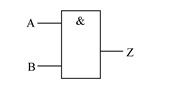
\includegraphics[width=1.78125in,height=0.96875in]{png-jpeg-pics/6AE5A9793FA0116A4D45F1A16270088B.png}\\
}

说明:当所有输入同时为``1''电平时,输出才为``1''电平,否则输出为``0''电平,见下表。

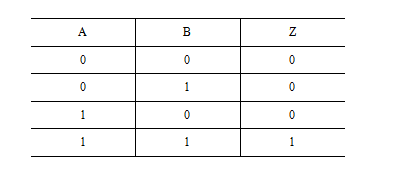
\includegraphics[width=4.30208in,height=1.76042in]{png-jpeg-pics/DA408AA7FED02B9C1B2633C900432551.png}

\textbf{(2)或门(有真即真)}

\textbf{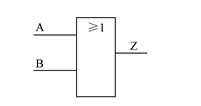
\includegraphics[width=2.09375in,height=1.10417in]{png-jpeg-pics/0A256D214CCCBE7B49FCE20794D709D4.png}\\
}

说明:多个输入端只要有一个输入端为``1''电平,输出就为``1''电平,只有所有输入端同时为``0''电平,输出才为``0''电平,见下表。

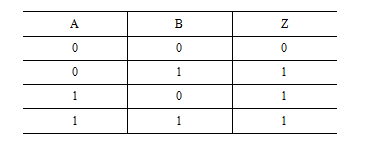
\includegraphics[width=3.84375in,height=1.50000in]{png-jpeg-pics/AB0DE573A20905AF9A0706947114536D.png}

\textbf{(3)非门(取反运算)}

\textbf{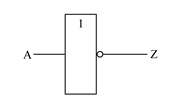
\includegraphics[width=2.01042in,height=1.06250in]{png-jpeg-pics/8627D3244B0E860C7C65D99E20C1530C.png}\\
}

说明:输入``1''电平,输出``0''电平;输入``0''电平,输出``1''电平(图中小圈表示取反),见下表。

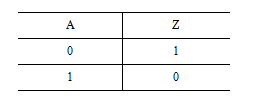
\includegraphics[width=2.66667in,height=1.09375in]{png-jpeg-pics/1535D421BF89ACB5B14E24DCA067C2FA.png}

\textbf{(}{\textbf{4}}{\textbf{)}}\textbf{或非门}

\textbf{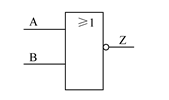
\includegraphics[width=1.76042in,height=1.04167in]{png-jpeg-pics/D079595E56F2D3CB2F78C23936D44790.png}\\
}

说明:和``或''门基本一样,只是将结果取反而已(图中小圈表示取反),见下表。

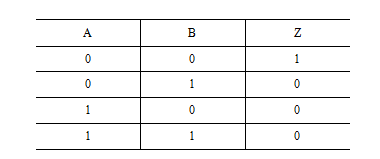
\includegraphics[width=3.95833in,height=1.65625in]{png-jpeg-pics/FB3022CE90E7192C26CB9F14823D7670.png}

\textbf{(}{\textbf{5}}{\textbf{)}}\textbf{与非门}

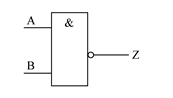
\includegraphics[width=1.80208in,height=1.02083in]{png-jpeg-pics/2E17F84C335C2A64461F0AC131328919.png}

说明:和``与''门基本一样,只是将结果取反而已,见下表。

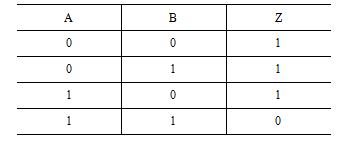
\includegraphics[width=3.79167in,height=1.53125in]{png-jpeg-pics/49990617AA06F48B25F8E30E91AE7C87.png}

\textbf{(}{\textbf{6}}{\textbf{)}}\textbf{异或门}

\textbf{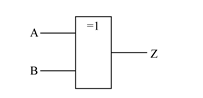
\includegraphics[width=2.11458in,height=1.02083in]{png-jpeg-pics/F1D7924BCB9866CBE0EA1D40F7786A5E.png}\\
}

说明:输入电平相同时,输出``0''电平;输入电平不同时,输出``1''电平。助记:同号相乘为正(0),异号相乘为负(1)。第2章介绍乘法符号的处理时会用到``异或''门,见下表。

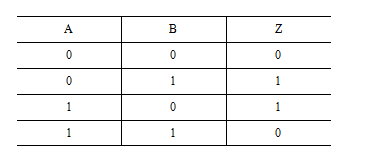
\includegraphics[width=3.83333in,height=1.65625in]{png-jpeg-pics/61F80E6C7CEDC5C8ADE5A753CCC9271C.png}

{注意:在输入端当然也可以使用小圈,只要记住图中小圈表示取反即可。}

\subsection{\texorpdfstring{{入门知识2}{:三态门}}{入门知识2:三态门}}\label{ux5165ux95e8ux77e5ux8bc62ux4e09ux6001ux95e8}

\textbf{三态门:}指逻辑门的输出端除有高、低电平两种状态外,还有第3种状态------高阻态(电路图参考下图)。高阻态相当于隔断状态(因为实际电路中不可能去断开它,所以设置这样一个状态,使它处于隔断状态),\textbf{例如,}内存中的一个存储单元,当读写控制线处于低电平时,存储单元被打开,可以写入数据;当处于高电平时,可以读出数据;但不读不写时,就要用高阻态,就像把该存储单元隔离开来一样。更直白的解释是,\textbf{高阻态}就是一个开关,当处于高阻态时,逻辑门什么也不能做。

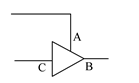
\includegraphics[width=1.44792in,height=0.86458in]{png-jpeg-pics/1A36DC3D965B35D598C8B9358E05D23A.png}

说明:当A为高电平时,C→B导通;当A为低电平时,C→B不导通,此时为高阻态。

\subsection{\texorpdfstring{{入门知识3}{:片选译码器}}{入门知识3:片选译码器}}\label{ux5165ux95e8ux77e5ux8bc63ux7247ux9009ux8bd1ux7801ux5668}

该知识点主要介绍最常用的3-8译码器(或称74138译码器,属于存储器与CPU连接中的片选译码器),其他的译码器(如2-4译码器、4-16译码器)原理都相似。常用的3-8译码器如下图所示:

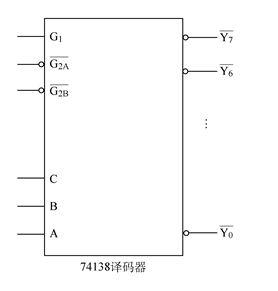
\includegraphics[width=2.89583in,height=3.03125in]{png-jpeg-pics/65104586957731D9682662843438BA6B.png}

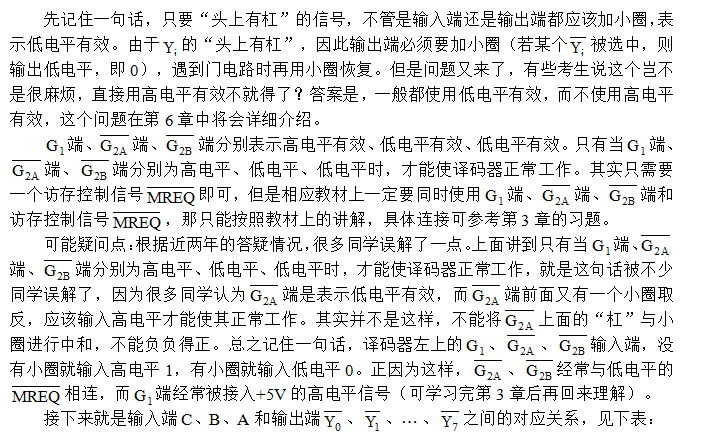
\includegraphics[width=3.70833in,height=2.29167in]{png-jpeg-pics/91C84C51CABCAAD6E19945EA4870BE74.png}\\
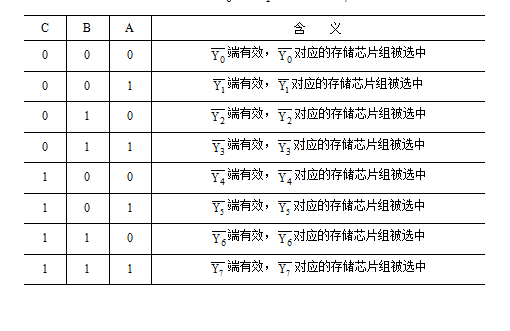
\includegraphics[width=3.70833in,height=2.40625in]{png-jpeg-pics/3DA4369AE81F8AFFF754C71BC6D1C3D4.png}

\textbf{{入门知识4:那些可怕的专业术语}}

\textbf{(1)系列机}

系列机是指一个厂家生产的具有相同系统结构、不同组成和实现的一系列不同型号的机器。它应在指令系统、数据格式、字符编码、中断系统、控制方式、输入/输出控制方式等方面保持统一,从而保证软件的兼容性。

\textbf{(2)阿姆代尔定律(Amdahl's ~Law)}

阿姆代尔定律是指系统优化某部件所获得的系统性能的改善程度,取决于该部件被使用的频率,或占用总执行时间的比例。该定律很好地刻画了改善``系统瓶颈''性能的重要性。

\textbf{(3)基准测试程序}

基准测试程序是专门用来进行性能评价的一组程序,这些程序能够很好地反映机器在运行实际负载时的性能。可以在不同机器上运行相同的基准测试程序来比较不同机器的运行时间,从而比较其性能。

\textbf{(4)最低有效位、最高有效位、最低有效字节、最高有效字节}

最低有效位:一个二进制数中的最低位,例如二进制数1110中的``0''。\\
最高有效位:一个二进制数中的最高位,例如二进制数0111中的``0''。\\
最低有效字节:一个二进制数中的最低字节,例如二进制数1111 1111 0000 0000
1111 0000中的``1111 0000''。\\
最高有效字节:一个二进制数中的最高字节,例如二进制数1111 1111 0000 0000
1111 0000中的``1111 1111''。

\textbf{(5)基数}

若进位计数制的``基数''为R,第n位数的权即Rn-1,则只要将各位数字与它的权相乘,并将其积累加,和数就是十进制数,例如,二进制数的基数是``2'',十进制数的基数为``10'',十六进制的基数为``16''。

\textbf{(6)逻辑数据}

逻辑数据用来表示命题的``真''和``假'',分别用``1''和``0''来表示。进行逻辑运算时,应按位进行。\\
{}

\subsection{\texorpdfstring{{入门知识}{5}{:与存储相关的那些名词}}{入门知识5:与存储相关的那些名词}}\label{ux5165ux95e8ux77e5ux8bc65ux4e0eux5b58ux50a8ux76f8ux5173ux7684ux90a3ux4e9bux540dux8bcd}

{有关存储的概念类包含存储元、存储单元、存储体、存储字和存储字长等,见下表。}

\textbf{情景助记:}假设将医院的整个住院部看成一个存储体,住院部由一个个病房组成(假设每个病房的床位数量都相等),那么每个病房就是一个存储单元,病房中的每张床就是一个存储元,每个病房的床位数量就是存储字长。\\
现假设病床上躺的都是0和1,而每间病房肯定都对应一串二进制代码。如果某病房二进制代码为10001000,则这串二进制代码可表示为十进制数136,也可以表示为十六进制数88H,当然也直接可以代表8位的二进制数。综上所述,可以将每个存储单元中二进制代码的组合看。

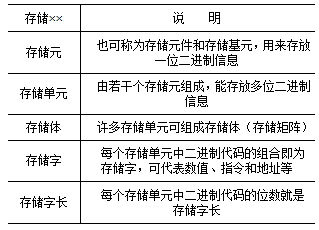
\includegraphics[width=3.32292in,height=2.39583in]{png-jpeg-pics/FC0C09D9C1D6B8FA4AF02309C41F2895.png}

\subsection{\texorpdfstring{{入门知识6}{:与字、字长相关的那些名词}}{入门知识6:与字、字长相关的那些名词}}\label{ux5165ux95e8ux77e5ux8bc66ux4e0eux5b57ux5b57ux957fux76f8ux5173ux7684ux90a3ux4e9bux540dux8bcd}

\subsection{\texorpdfstring{{1B=8bit,这个是规定,没有错误。但是很多考生认为一个字等于两个字节,因为他们脑海中有一种概念:一个汉字占用两个字节。计算机中的字和汉字中的字的概念不一样。计算机中的字通常由一个或多个(一般是字节的整数倍)字节构成。现在常用的都是32位(4个字节)字长的机器。}}{1B=8bit,这个是规定,没有错误。但是很多考生认为一个字等于两个字节,因为他们脑海中有一种概念:一个汉字占用两个字节。计算机中的字和汉字中的字的概念不一样。计算机中的字通常由一个或多个(一般是字节的整数倍)字节构成。现在常用的都是32位(4个字节)字长的机器。}}\label{b8bitux8fd9ux4e2aux662fux89c4ux5b9aux6ca1ux6709ux9519ux8befux4f46ux662fux5f88ux591aux8003ux751fux8ba4ux4e3aux4e00ux4e2aux5b57ux7b49ux4e8eux4e24ux4e2aux5b57ux8282ux56e0ux4e3aux4ed6ux4eecux8111ux6d77ux4e2dux6709ux4e00ux79cdux6982ux5ff5ux4e00ux4e2aux6c49ux5b57ux5360ux7528ux4e24ux4e2aux5b57ux8282ux8ba1ux7b97ux673aux4e2dux7684ux5b57ux548cux6c49ux5b57ux4e2dux7684ux5b57ux7684ux6982ux5ff5ux4e0dux4e00ux6837ux8ba1ux7b97ux673aux4e2dux7684ux5b57ux901aux5e38ux7531ux4e00ux4e2aux6216ux591aux4e2aux4e00ux822cux662fux5b57ux8282ux7684ux6574ux6570ux500dux5b57ux8282ux6784ux6210ux73b0ux5728ux5e38ux7528ux7684ux90fdux662f32ux4f4d4ux4e2aux5b57ux8282ux5b57ux957fux7684ux673aux5668}

\subsection{\texorpdfstring{{以前是存储字长等于机器字长,因为机器字长是机器一次能处理的比特数,这样一次取一个等长的存储字便于机器处理。现在机器字长一般大于存储字长。}}{以前是存储字长等于机器字长,因为机器字长是机器一次能处理的比特数,这样一次取一个等长的存储字便于机器处理。现在机器字长一般大于存储字长。}}\label{ux4ee5ux524dux662fux5b58ux50a8ux5b57ux957fux7b49ux4e8eux673aux5668ux5b57ux957fux56e0ux4e3aux673aux5668ux5b57ux957fux662fux673aux5668ux4e00ux6b21ux80fdux5904ux7406ux7684ux6bd4ux7279ux6570ux8fd9ux6837ux4e00ux6b21ux53d6ux4e00ux4e2aux7b49ux957fux7684ux5b58ux50a8ux5b57ux4fbfux4e8eux673aux5668ux5904ux7406ux73b0ux5728ux673aux5668ux5b57ux957fux4e00ux822cux5927ux4e8eux5b58ux50a8ux5b57ux957f}

\subsection{\texorpdfstring{{\textbf{一般默认字长=机器字长=存储字长}。}}{一般默认字长=机器字长=存储字长。}}\label{ux4e00ux822cux9ed8ux8ba4ux5b57ux957fux673aux5668ux5b57ux957fux5b58ux50a8ux5b57ux957f}

\subsection{\texorpdfstring{{\textbf{入门知识7}}{\textbf{:与周期相关的那些名词}}}{入门知识7:与周期相关的那些名词}}\label{ux5165ux95e8ux77e5ux8bc67ux4e0eux5468ux671fux76f8ux5173ux7684ux90a3ux4e9bux540dux8bcd}

{有关周期的概念主要有以下几种,见下表}

{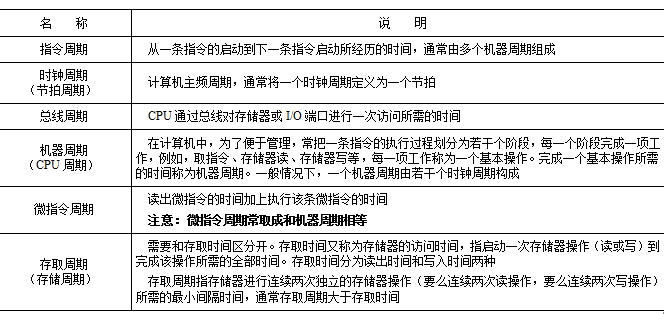
\includegraphics[width=3.69792in,height=1.75000in]{png-jpeg-pics/6EA31B167B4F1FE19AFEBA0749A267DD.png}\\
}
